% This is LLNCS.DEM the demonstration file of
% the LaTeX macro package from Springer-Verlag
% for Lecture Notes in Computer Science,
% version 2.4 for LaTeX2e as of 16. April 2010
%
\documentclass{llncs}
%
%\usepackage{makeidx}  % allows for indexgeneration
\usepackage{wrapfig}
\usepackage{float}
\usepackage[english]{babel}
\usepackage{lipsum}
\usepackage{caption}
\usepackage{subcaption}
\usepackage{graphicx}
	\graphicspath{{images/}} 
%\usepackage{cite}
\usepackage[linesnumbered,ruled]{algorithm2e}
\usepackage{courier}
\usepackage{hyperref}
    \hypersetup{colorlinks=true,allcolors=blue}
\usepackage{listings}
	\lstset{
  		basicstyle=\ttfamily,
  		frame=none, 
  		breaklines=true,
  		numbers=left,
  		xleftmargin=2.5em,
  		framexleftmargin=0em,
    	emphstyle=\textbf,
    	float=t
	}
	\lstdefinestyle{ocl}{
  		emph={
        	context, inv
    	}
	}
	\lstdefinestyle{cbp}{
	    basicstyle=\ttfamily\scriptsize,
  		emph={
        	session, create, of, type,
        	set, to, add, hire
    	}
	}
	\lstdefinestyle{xmi}{
		basicstyle=\ttfamily\scriptsize,
  		emph={
        	Node, children
    	}
	}
	\lstdefinestyle{xml}{
	    basicstyle=\ttfamily\scriptsize,
  		emph={
        	register, create, add, to, resource,
        	from, eattribute, remove, ereference,
        	set, unset, session, Roy, Jen,
        	Moss, Richmond
    	}
	}
	\lstdefinestyle{java}{
	    basicstyle=\ttfamily\scriptsize,
  		emph={
        	case, UNSET,
        	instanceof, else, if, void,
        	new, UnsetEAttributeEvent,
        	UnsetEReferenceEvent,
        	@override, public, class, extends
    	}
	}
	\lstdefinestyle{eol}{
	    basicstyle=\ttfamily\scriptsize,
  		emph={
        	var, new, for, in, create, set, of, with, 
        	unset, to, add, remove, delete, register,
        	from, position, from, move-within, session, \.
    	}
	}

\begin{document}
\renewcommand{\thelstlisting}{\arabic{lstlisting}}
\renewcommand{\labelitemi}{$\bullet$}
\newcommand{\dk}[1]{\textbf{[DK: #1]}}

\title{An Algorithm for Efficient Loading \\ of Change-Based Models}
%
%\titlerunning{Change-based Persistence and Its Loading Optimisation}  % abbreviated title (for running head)
%                                     also used for the TOC unless
%                                     \toctitle is used
%
\author{
    Anonym%Alfa Yohannis \and Dimitris Kolovos \and Fiona Polack 
}
%
\authorrunning{
    Anonym%Alfa Yohannis et al.
} % abbreviated author list (for running head)
%
%%%% list of authors for the TOC (use if author list has to be modified)
%\tocauthor{Dimitris Kolovos, Fiona Polack, Alfa Yohannis}
%

\institute{anonym}
%\institute{Department of Computer Science, University of York, United Kingdom\\
%\email{\{ary506, dimitris.kolovos, fiona.polack\}@york.ac.uk}}

\maketitle              % typeset the title of the contribution
%The first states the problem. The second states why the problem is a problem. The third is my startling sentence. The fourth states the implication of my startling sentence.
\begin{abstract}
The benefits obtained from using changed-based persistence (CBP) for object-oriented (MOF/Ecore) models comes at the cost of increased load costs. The additional cost can outweigh the benefits and as a result CBP may not be widely adopted. By providing an optimized loading mechanism the load times of CBP can be improved. By reducing the load times, CBP will be widely adopted and allow tools to provide better collaborative modelling environments, support faster incremental model validation and transformation, among others. Our results show show that the proposed optimizations can improve loading times up to 80\% compared to the original CBP; further, the results show improved store performance against the existing CBP solution while preserving constant store times.

Recent work introduced a language-independent change-based format for persisting models in object-oriented metamodelling architectures such as MOF and EMF. In this format, instead of the state of a model, its full change history model is persisted instead, and the state of the model is reconstructed at loading time by replaying this history. In this paper, we contribute a more efficient algorithm for loading such models. The proposed algorithm detects and skips changes that are superseded by later changes -- and which therefore have no impact to the eventual state of the model. We evaluate the performance of the new loading algorithm experimentally and we assess its memory footprint and the impact it has on saving change-based models. 

\end{abstract}

\section{Introduction}
\label{sec:introduction}
Existing approaches for file-based persistence of models in metamodelling architectures such as MOF and EMF are predominately state-based. In such approaches, model files contain snapshots of the models' contents and activities such as version control and change detection are left to external systems such as file-based version-control systems and model differencing facilities. Activities such as model comparison and change detection are computationally consuming for state-based models and can become a burden as larger models are developed in a collaborative setting. 

In contrast to persisting the \emph{states} of models, we harness a change-based approach that persists the full sequence of \emph{changes} made to models instead. The change-based approach comes with a number of envisioned benefits over stated-based persistence, such as the ability to detect changes much faster and more precisely \cite{yohannis2017turning}, which can then have positive knock-on effects on helping developers to diff/merge models in collaborative modelling environments, as well as supporting faster incremental model validation and transformation \cite{rath2012derived}, \cite{ogunyomi2015property}. However, change-based persistence comes with a downside---an increased load cost---since all recorded changes need to be replayed to reconstruct a model's state \cite{yohannis2017turning}.   

Our work extends the previous work of Yohannis et al. \cite{yohannis2017turning} that implements a change-based persistence (CBP) format by proposing and evaluating an algorithm that reduces loading time of change-based models by avoiding replaying changes that have no impact on the eventual state of the model (e.g. that are cancelled out by subsequent changes). We assess the efficiency of the algorithm in terms of persistence and loading time, and memory footprint. Our approach demonstrates considerable savings in time for persisting changes made to models, at a higher, but linear, model loading cost, compared to state-based models when tested on large scale models. %\dk{If the contribution we're proposing in this paper is the optimised loading algorithm, starting that loading cost is higher can be confusing.}

The rest of the paper is structured as follows. Section \ref{sec:case_study} introduces a running example and provides a brief overview of the change-based model persistence we extend. Section \ref{sec:loading_time_optimisation} presents an algorithm that intends to speed up loading of change-based models, and its supporting data structures. %\dk{Merge Sections 3 and 4}.  
Sect. \ref{sec:performance_evaluation} shows the results of controlled evaluation experiments for assessing the benefits of the proposed algorithm. Section \ref{sec:related_work} provides an overview of existing related work. Section \ref{sec:limitations_and_future_work} discusses the limitations of our approach and potential future work, and Sect. \ref{sec:conclusions} concludes this paper.

\begin{figure}[b]
    \begin{subfigure}[t]{0.4\linewidth}
        \centering
        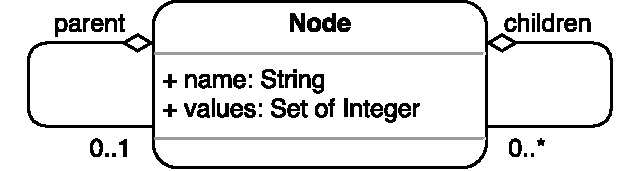
\includegraphics[width=0.8\linewidth]{node_metamodel}
        \caption{The tree metamodel.}
        \label{fig:tree_metamodel}
    \end{subfigure}
    \hfill
    \begin{subfigure}[t]{0.6\linewidth}
        \centering
        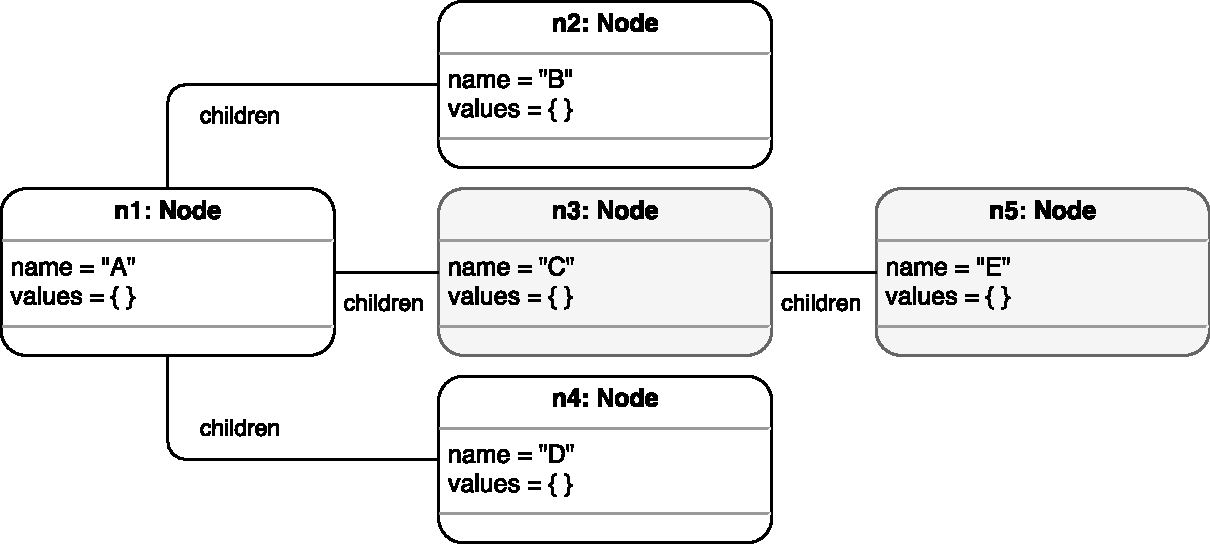
\includegraphics[width=\linewidth]{initial_chart}
        \caption{A model that conforms to the tree metamodel (n3 was created and then deleted)}
        \label{fig:initial_model}
    \end{subfigure}
    \caption{A tree metamodel and its model as the running example.}
    \label{fig:append_speed}
\end{figure}

\section{Running Example}
\label{sec:case_study}
To explain the proposed algorithm, we use the minimal tree metamodel and model illustrated in Figures \ref{fig:tree_metamodel} and \ref{fig:initial_model}. We chose this example to avoid unnecessary repetition in our discussion, while providing a reasonable coverage of the basic features of the Ecore metamodelling language (classes, single/multi-valued features, references and attributes). In our example, tree models consist of named nodes which can -- optionally -- contain other nodes (\emph{children} reference).

The model in Fig. \ref{fig:initial_model} consists of two nodes \emph{n1}, \emph{n2}. To construct this model, we started by creating and naming three nodes (\emph{n1}, \emph{n2} and \emph{n3}). Nodes \emph{n2} and \emph{n3} were then added as children of \emph{n1}. Finally, node \emph{n3} was deleted from the model. The state of the resulting model is illustrated in simplified XMI in Listing \ref{lst:xmimodel}.

\noindent
\begin{minipage}[t]{0.34\linewidth}
\begin{lstlisting}[style=xmi,caption={State-based representation of the tree model in (simplified) XMI.},label=lst:xmimodel]
<Node id="n1" name="A">
  <children id="n2" 
    name="B"/>
</Node>
\end{lstlisting}
\end{minipage}
\hfill
\begin{minipage}[t]{0.635\linewidth}
\begin{lstlisting}[style=eol,caption={Change-based representation of the tree model.},label=lst:cbpmodel]
create n1 of Node
set n1.name to "A"      
create n2 of Node
set n2.name to "B"      
create n3 of Node
set n3.name to "C"      
add n2 to n1.children   
add n3 to n1.children
remove n3 from n1.children   
delete n3
\end{lstlisting}
\end{minipage}

In contrast to the state-based representation, a CBP representation of the model is illustrated in Listing \ref{lst:cbpmodel} (the syntax is a simplified version of the one introduced in\,\cite{yohannis2017turning} ).
Lines 1-6 record the creation and naming of the three nodes, lines 7 and 8 record the addition of \emph{n2} and \emph{n3} as children of \emph{n1} and lines 9-10 captures the deletion of \emph{n3} (deletion effectively involves two events).

% Instead of treating the model as a state based, we records all events generated by the the consecutive  operations and persist them into a CBP representation (Listing \ref{lst:cbpmodel}), which contains at least as much information as the state-based representation. Replaying all these events produces the same state as the one captured in the Listing \ref{lst:xmimodel}.  

For a large model, this approach is beneficial since we only need to persist the events as opposed to the entire model.
However, loading the model by reapplying all the events\,\cite{yohannis2017turning}  is not efficient.
The inefficiency is the result of applying events that are cancelled out by subsequent events.
For example,  creating \emph{n3} at line 5 and adding it to the children of \emph{n1} at line 8 are cancelled by the deletion of \emph{n3} at line 9.
The events at lines 5, 9 and 10 are \emph{unnecessary}.
%An optimisation can be performed by ignoring the unnecessary events. For example, the deletion of node \emph{n3} makes events (Listing \ref{lst:xmimodel}, lines 5-6, 8-10) related to the node unnecessary to be replayed. 

\section{Loading Time Optimisation}

THE FIGURE IS NOT CLEAR, DONT UNDERSTAND THE ARROWS OF THE DIFFERENCE IN THE SHAPES.

\label{sec:loading_time_optimisation}
Figure \ref{fig:flowchart} illustrates the context of our work, when and where we use the proposed algorithm to optimise the loading of CBP. 

\begin{figure}[ht]
\centering
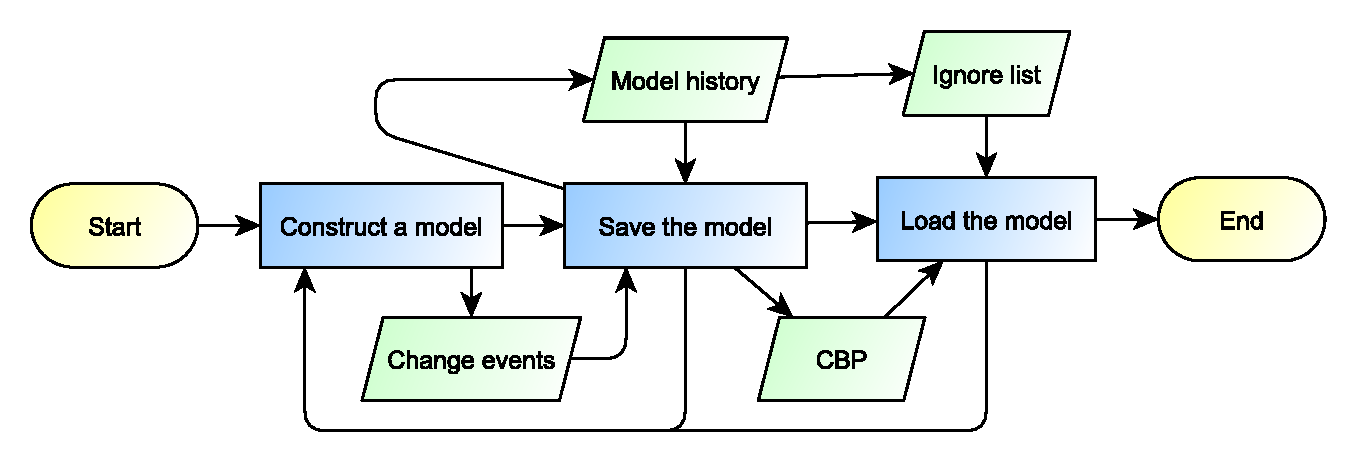
\includegraphics[width=\linewidth]{flowchart}
\caption{The context flowchart of optimising loading performance of CBP.}
\label{fig:flowchart}
\end{figure}

During the construction of a model by an agent (i.e. man, software), all the relevant events for CBP are captured and put into a list of change events. When the agent saves the model, the saving process persists all the change events into a CBP representation. While iterating through all the change events to append each of them into the CBP, a model history is populated (the model history is explained in the following subsection). The proposed algorithm is executed and uses the model history as a ``memory" to determine the unnecessary events---events that can be ignored when loading the CBP. The event numbers of the unnecessary events are put into an ignore list and then persisted. 

CBP that already saved can be reloaded to continue the construction of the model. In loading the CBP, the loading process reload the ignore list first and use it as a reference to determine which events in the CBP that do not need to be replayed. If the event number of an event in the CBP exists in the ignore list then the event can be ignored and the load process can continue to subsequent events. 

\subsection{Model History}
The proposed algorithm uses a data structure that memorises elements' events and their position (line number) in a CBP representation so it can reason about the events of a particular element and determine which are cancelled out.
For the rest of the discussions the line number in the CBP representation is referred to as the \emph{event number}. The proposed data structure is presented in figure \ref{fig:object_history} as a class diagram.  

THE EVENT HISTORY SHOULD ONLY HAVE ONE Line
ElementHistory HAS THE IsMoved FLAG BUT THE ALGORITHMS USE THE isFeatureMoved... why?

\begin{figure}[ht]
\centering
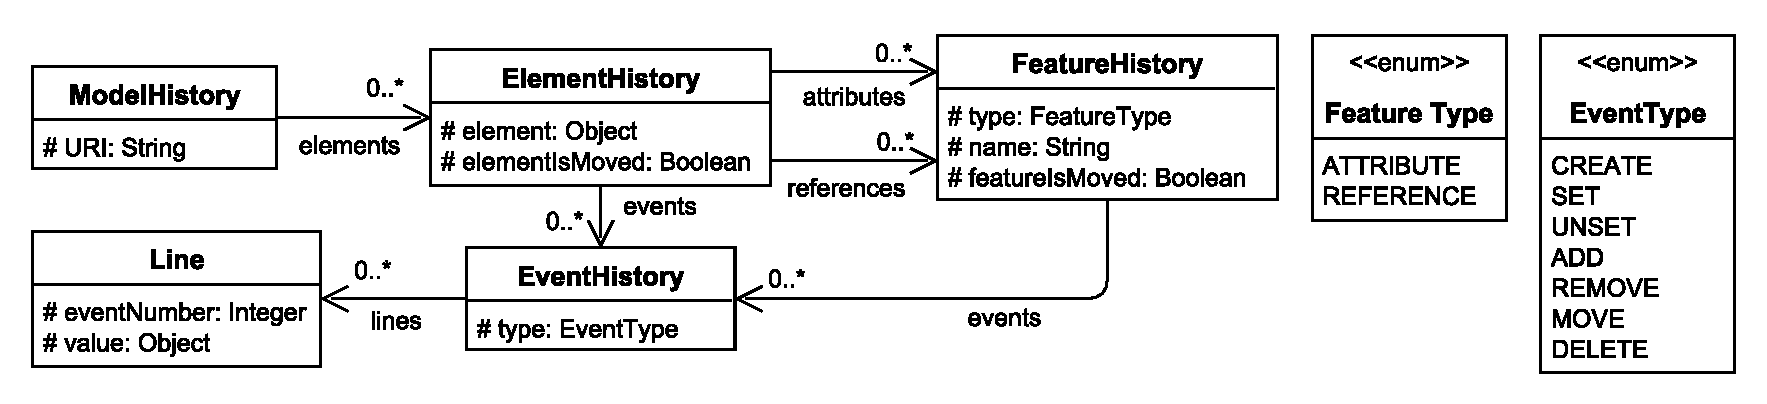
\includegraphics[width=\linewidth]{object_history}
\caption{The class diagram of model history.}
\label{fig:object_history}
\end{figure}

\begin{figure}[ht]
\centering
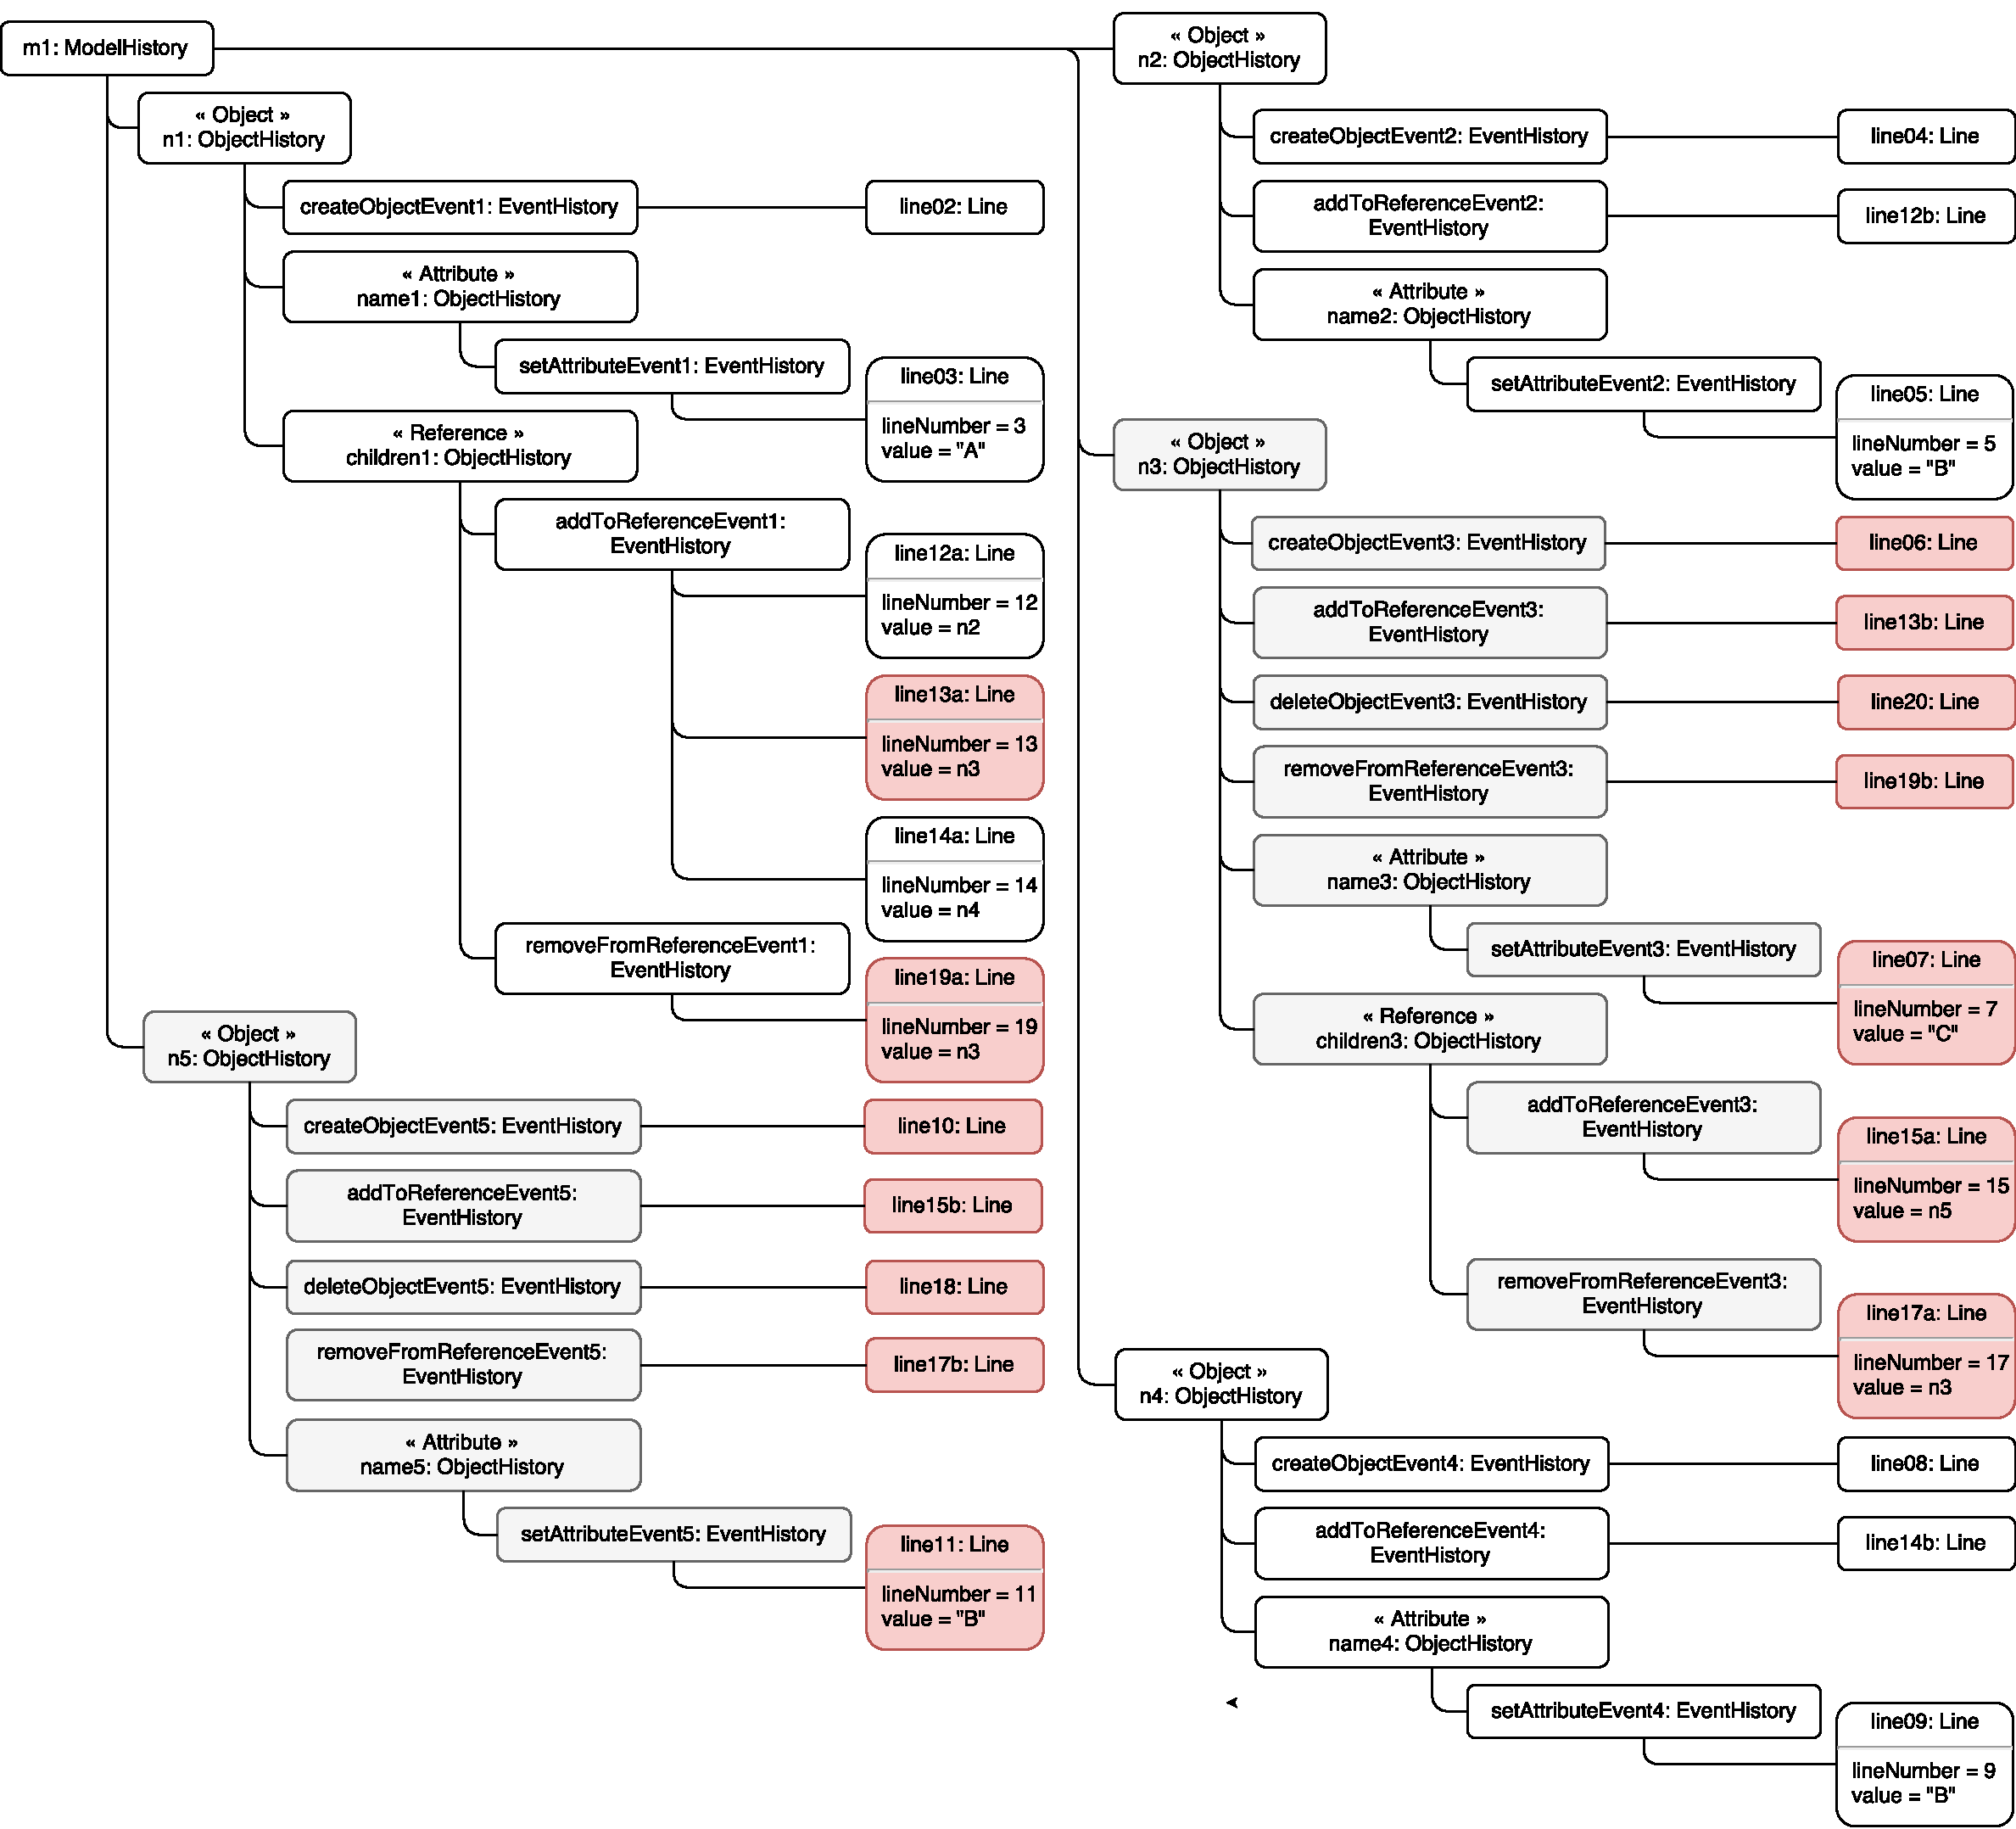
\includegraphics[width=\linewidth]{history_structure}
\caption{The object diagram of model history of the CBP in Listing \ref{lst:cbpmodel}.}
\label{fig:history_structure}
\end{figure}

A \emph{ModelHistory} has attribute \emph{URI} to identify the model for which it records changes and can have many \emph{ElementHistory} elements.
An \emph{ElementHistory} has an attribute \emph{element} that identifies the element that it refers to and a \emph{isMoved} is flag.
The  \emph{isMoved} flag is used to indicate a \emph{move} event for the element (section \ref{subsec:add_remove_and_move_operations} provides details of its use).
Every \emph{ElementHistory} can have many \emph{FeatureStory} to represent features of an element that are used in the CBP.  	%that are involved in certain events (i.e. ``\emph{add n2 to n1.children}" event has the \emph{children} as the feature).
A \emph{FeatureHistory} has two attributes \emph{type} to identify its type (attribute or reference) and \emph{name} to identify the feature's name.

An \emph{EventHistory} represents an event in the CBP model.
An \emph{EventHistory} has an attribute \emph{type} to identify the event's type and can have many \emph{Line}s.
A \emph{Line} has an \emph{eventNumber} attribute to store the line number in the CBP model and a \emph{value} that is used to store the element involved in the event (it is only used for ADD, REMOVE and MOVE events)

Each \emph{FeatureStory} can have many \emph{EventHistory}s  to represent the events that modify the value of the feature.
Each \emph{ElementHistory}  can have many \emph{EventHistory}s to represent events that affect the state of the element (life-cycle and relations to multivalued features).
%For events that involve the element individually (e.g. create, add) element's feature but only affect the element (i.e. ``\emph{create n1 of Node}" event has no feature involved), or events in which an element acts as an operand for a multi-valued feature (i.e. ``\emph{add n3 to n1.children}" event has the \emph{n3} as the operand).
%These kinds of events can have their \emph{EventHistory} belong to their \emph{ElementHistory} directly.

Figure \ref{fig:history_structure} shows the object diagram of the model history of the CBP model in Listing \ref{lst:cbpmodel} (some attribute values are not shown).
The grey rectangles are \emph{*History} objects of that belong to the deleted node \emph{n3}.
The red rectangles are \emph{Line} objects that represent unnecessary events.

Next, we present the algorithms that use the information stored in the model history to identify events that have no impact in the final state of the model, i.e. the unnecessary events.
The algorithms produce the Ignore Lists that are used to optimize the CBP loading algorithm.
WE ARE MISSING SOMETHING THAT SAYS HOW EACH ALGORITHM IS INVOKED FOR EACH FEATURE/ELEMENT AND THAT THE COMPLETE IGNORE LIST IS THE UNION OF ALL IGNORE LSITS?

\begin{lstlisting}[style=eol,caption={The CBP representation of attribute \emph{name} assignments.},label=lst:set_unset_example]
create n1 of Node
set n1.name to "A"
unset n1.name
set n1.name to "B"
\end{lstlisting}

\subsection{Set and Unset Events}
\label{subsec:set_and_unset_events}
While working on a model, a single-valued feature can be assigned many times.
Each of the assignments is persisted as an event in the CBP model.
Only the last assigned value is necessary to obtain the final state of the feature. 
That is, all events but the last can be ignored.
For example in Listing \ref{lst:set_unset_example}, the feature \emph{name} is assigned the ``A" value, nullified (unset), and finally assigned the ``B" value.
That is, in the last state of the model: \emph{n1.name = ``B"}.
As a result, the load process could ignore all previous events and only replay the last assignment event (line 4). 
%\noindent
%\begin{minipage}[t]{0.49\linewidth}

%\end{minipage}
%\hfill
%\begin{minipage}[t]{0.49\linewidth}
%\begin{lstlisting}[style=eol,caption={The CBP representation of reference  \emph{parent} assignments.},label=lst:set_unset_reference]
%create n1 of Node
%create n2 of Node
%create n3 of Node
%set n3.parent to n1
%set n3.parent to n2
%unset n3.parent
%\end{lstlisting}
%\end{minipage}

\begin{algorithm}[H]
\begin{small}
\SetKwInOut{Input}{input}
\SetKwInOut{Output}{output}
\Input{two lists of Integer $setEventNumbers$}
\Output{a list of Integer $ignoreList$}
\SetKwBlock{Beginn}{beginn}{ende}
\Begin{
$setLastLine$ $\leftarrow$ getLastLine($setEventNumbers$)\;
$unsetLastLine$ $\leftarrow$ getLastLine($unsetEventNumbers$)\;
\uIf{$setLastLine > unsetLastLine$}{
    $ignoreList \leftarrow (setEventNumbers \cup unsetEventNumbers) \setminus \{setLastLine\} $\;
}
\ElseIf{$setLastLine < unsetLastLine$}{
    $ignoreList \leftarrow (setEventNumbers \cup unsetEventNumbers)$\;
}
\Return{$ignoreList$}\;
}
\end{small}
\caption{Algorithm to identify event numbers of unnecessary \emph{set} and \emph{unset} events}
\label{alg:set_unset_optimisation}
\end{algorithm}

The algorithm that identifies unnecessary \emph{SET} and \emph{UNSET} events for a feature is presented in Alg. \ref{alg:set_unset_optimisation}.
The algorithm has two inputs: a list of event numbers of \emph{SET} events and a list of event numbers of \emph{UNSET} events.
The output of the algorithm is an \emph{ignoreList} that includes the event numbers that are unnecessary.
The inputs lists can be easily constructed from the model history data structure.
For the \emph{name} feature in Listing \ref{lst:set_unset_example} these are: $setEventNumbers = \{2,4\}$ and $unsetEventNumbers = \{3\}$.

The \emph{ignoreList} is populated as follows.
In lines 4 and 5, the last event number of each input list is stored in \emph{setLastLine} and \emph{unsetLastLine} respectively.
If $setLastLine > unsetLastLine$ (line 7) then $ignoreList = (setEventNumbers \cup unsetEventNumbers) \setminus  \{setLastLine\} $, i.e. all events except the last \emph{SET} event can be ignored.
If $setLastLine > unsetLastLine$ (line 9) then $ignoreList = (setEventNumbers \cup unsetEventNumbers)$, i.e. all events can be ignored.

For the \emph{name} feature in Listing \ref{lst:set_unset_example} $ignoreList = \{2, 3\}$.

\subsection{Add, Remove, and Move Events}\label{subsec:add_remove_and_move_operations}
DO WE SAY HERE THAT THE LIMITATION IS THAT IT ONLY WORKS IN UNIQUE COLLECTIONS?

While working on a model, the contents of a multi-valued feature can be modified many times.
If the same element is added and removed multiple times,  only that last event is necessary to determine if the element should appear in the multi-valued feature values in the final state of the feature.
For example in Listing \ref{lst:add_remove_move_reference},  nodes \emph{n2} and \emph{n3} are added to the \emph{children} feature of \emph{n1} (lines 4-5), and then \emph{n3} is removed (line 6).
That is, in the last state of the model: \emph{n1.children = [n2]}.
As a result, the load process could ignore the events that represent the ADD and REMOVE events of \emph{n3}.

\begin{lstlisting}[style=eol,caption={Example of CBP representation of attribute \emph{values}'s add and remove operations.},label=lst:add_remove_move_reference]
create n1 of Node
create n2 of Node
create n3 of Node
add n2 to n1.children
add n3 to n1.children
remove n3 from n1.children
\end{lstlisting}

\begin{algorithm}[H]
\begin{small}
\SetKwInOut{Input}{input}
\SetKwInOut{Output}{output}
\SetKwProg{Struct}{struct}{}{end}
\Struct{Line}{
    Integer $eventNumber$;
    Anytype $value$;
}
\Input{two lists of Line $addEventLines$, $removeEventLines$, a variable of Anytype $operandValue$, a variable of Boolean $featureIsMoved$} % and $moveEventLines$, , an variable of Feature $feature$}
\Output{a list of Integer $ignoreList$}
\SetKwBlock{Beginn}{beginn}{ende}
\Begin{
\If{$featureIsMoved$ = false}{
    $filteredAddLines$ $\leftarrow$ filterByValue($addEventLines$, $operandValue$)\;
$filteredRemoveLines$ $\leftarrow$ filterByValue($removeEventLines$, $operandValue$)\;
$addLastLine$ $\leftarrow$ getLastLine($filteredAddLines$)\;
$removeLastLine$ $\leftarrow$ getLastLine($filteredRemoveLines$)\;
\uIf{$addLastLine > removeLastLine$}{
     $ignoreList \leftarrow (filteredAddLines.eventNumber \cup filteredRemoveLines.eventNumber \setminus \{addLastLine\} $\;
}
\ElseIf{$addLastLine < removeLastLine$}{
    $ignoreList \leftarrow (filteredAddLines.eventNumber \cup filteredRemoveLines.eventNumber$\;
}
}
%\If{feature is empty}{
%       Add all event numbers in $addEventLines$, $removeEventLines$, and $moveEventLines$ into $ignoreList$\;
%        $attributeIsMoved$ $\leftarrow$ false\;
%}
\Return{$ignoreList$}\;
}
\end{small}
\caption{Algorithm to identify event numbers of unnecessary \emph{add}, \emph{remove}, and \emph{move} events.}
\label{alg:add_remove_move_optimisation}
\end{algorithm}

I REMOVED THE "feature is empty" CONDITION BECAUSE IT COMPLICATES THE EXPLANATION AND DOES NOT ADD TO THE DISCUSSION. FURTHER, THE UNION OF ALL IGNORE LISTS WILL BE THE SAME AS THE UNION INSIDE THE CONDITION. 

The algorithm that identifies unnecessary \emph{ADD} and \emph{REMOVE} events for a feature is presented in Alg. \ref{alg:add_remove_move_optimisation}.
The algorithm has four inputs: a list of Line objects of \emph{ADD} events, a list of Line objects of \emph{REMOVE} events, the element of interest and a flag that indicates a MOVE event on the analysed feature. 
The output of the algorithm is an \emph{ignoreList} that includes the event numbers that are unnecessary.
The inputs lists can be easily constructed from the model history data structure.
For the \emph{children} feature in Listing \ref{lst:add_remove_move_reference} these are: $addEventLines = \{  \{4, n2 \}, \{5, n3 \} \}$, $removeEventLines = \{\{6, n3 \}\}$, $moveEventLines = \emptyset$,\linebreak $operandValue = n3$, and $featureIsMoved = \mathrm{False}$

The \emph{ignoreList} is populated as follows.
If the flag \emph{featureIsMoved} is True then nothing is added to the list (the need for this flag is explained later in this section).
If the flag \emph{featureIsMoved} is False, then lines 6 and 7 filter the $addEventLines$ and $removeEventLines$ so we only keep Lines for which the \emph{value} is equal to \emph{operandValue}.
The filtered lists are stored in $filteredAddLines$ and $filteredRemoveLines$ respectively.
The rest of the algorithm works similar to Alg. \ref{alg:set_unset_optimisation}, ignoring all events but the last if it was an ADD, else ignoring all events. 

%However, this logics can only be executed if there is no \emph{move} event has been applied to the feature (the reason is explained later in this section) and it is indicated by false value of the flag \emph{featureIsMoved} (line 5). That is why excluding \emph{moveEventLines} is excluded from filtering because no \emph{move} event has been made. The flag \emph{featureIsMoved} is set to true (false is the default value) when the first \emph{move} event is applied to the feature and is set back to false when the feature is empty or has no value. If the feature is empty then all event numbers in the \emph{addEventLines}, \emph{removeEventLines}, and \emph{moveEventLines} into the \emph{ignoreList}. After that, \emph{attributeIsMoved} is set to false. Finally, the \emph{ignoreList} is returned for further operations.

The flag \emph{featureIsMoved} at line 5 in Alg. \ref{alg:add_remove_move_optimisation} is required to prevent ordering errors in the final state.
Consider the example presented in Listing \ref{lst:move_attribute_example_error} and the optimised CBP model of Listing \ref{lst:move_attribute_example} which does not consider the \emph{featureIsMoved} flag.
In the optimized CBP model the events related to \emph{n2} have been ignored.
Notice that the final state of the optimized version is $p.values = [13, 11]$  which is different from the original version $p.values = [11,13]$.
The reason is that the move event at line 8 in the original version works of a different value that the one in the optimized version.

\begin{lstlisting}[style=eol,caption={The CBP representation of attribute \emph{values}'s move event.},label=lst:move_attribute_example]
create p of Node
create n1
create n2
create n3
add n1 to p.children
add n2 to p.children
add n3 to p.children
move from 0 to 1 in p.children
remove n2 from p.children
\end{lstlisting}

\begin{lstlisting}[style=eol,caption={The optimised CBP representation of attribute \emph{values}'s event.},label=lst:move_attribute_example_error]
create p of Node
create n1
create n2
create n3
add n1 to p.children
add n3 to p.children
move from 0 to 1 in p.children
\end{lstlisting}

\subsection{Create and Delete Events}
\label{subsec:create_and_delete_operations}
When an element is deleted, it means that the element is completely removed from the model.
Therefore, all events (create, set, unset, move, add, remove, delete) related to the element that happen before the event can be ignored, including all events related to its features (unless the element has been moved).
For example, when node \emph{n3} in Listing \ref{lst:cbpmodel}  is deleted, the events on lines 5-6 and 8-10 are unnecessary.
The optimised CBP model of Listing \ref{lst:cbpmodel} is presented in Listing \ref{lst:cbpmodel_optimised}.

\begin{lstlisting}[style=eol,caption={Change-based representation of the model of Figure \ref{fig:initial_model} after removal of node \emph{n5}.},label=lst:cbpmodel_optimised]
create n1 of Node
set n1.name to "A"
create n2 of Node
set n2.name to "B"
add n2 to n1.childre
\end{lstlisting}

\begin{algorithm}[H]
\begin{small}
\SetKwInOut{Input}{input}
\SetKwInOut{Output}{output}
\Input{a variable of Object $deletedElement$, a list of Integer $ignoreList$}
\Output{a list of Integer $ignoreList$}
\Begin{
$elementIsMoved$ $\leftarrow$ isElementMoved($deletedElement$)\;
\If{$elementIsMoved$ = false}{
    $eventHistoryList$ $\leftarrow$ getAllEventHistories($deletedElement$)\; 
    \ForEach{$eventHistory$ in $EventHistoryList$}{
        $lineList$ $\leftarrow$ getLines($eventHistory$)\;
        Add all event numbers in $lineList$ into $ignoreList$\; 
    }
    $featureList$ $\leftarrow$ getAllAttributes($deletedElement$)\;
    \ForEach{$attribute$ in $featureList$}{
        $eventHistoryList$ $\leftarrow$ getAllEventHistories($feature$)\;
        \ForEach{$eventHistory$ in $EventHistoryList$}{
            $lineList$ $\leftarrow$ getLines($eventHistory$)\;
            Add all event numbers in $lineList$ into $ignoreList$\; 
        }       
    }   
}
\Return{$ignoreList$}\;
}
\end{small}
\caption{Algorithm to identify lines that are ignored after \emph{delete} events}
\label{alg:create_delete_optimisation}
\end{algorithm}

The algorithm that identifies unnecessary events for a deleted element is presented in Alg. \ref{alg:create_delete_optimisation}.
The algorithm has one input: the deleted element.
The output of the algorithm is an \emph{ignoreList} that includes the event numbers that are unnecessary.
The inputs lists can be easily constructed from the model history data structure.

The algorithm starts by checking flag \emph{elementIsMoved} to determine whether the \emph{deletedElement} is already moved or not (line 2).
If it is false then it is safe to remove all lines that refer to the element (line 3) (the reason for use of the flag has been explained in subsection \ref{subsec:add_remove_and_move_operations}).
Otherwise, no action is executed.
The algorithm then retrieves all event histories \emph{eventHistoryList} that refer to the element (line 4) and iterates through each event history (line 5-8).
For every event history \emph{eventHistory} (line 5), the algorithm retrieves its lines \emph{lineList} (line 6) and put all their event numbers into the \emph{ignoreList} (line 7).
After that, the algorithm continues to iterate through all its features and put all lines' event numbers of their events into the \emph{ignoreList} (lines 12-15). Finally, the algorithm returns the \emph{ignoreList} as its output.


%The \emph{ignoreList} acts as a lookup reference when a CBP is loaded. If an event's event number is contained in the \emph{ignoreList}, the event is not replayed and the load process continue to the next event.


\section{Performance Evaluation}
\label{sec:performance_evaluation}
We have implemented a prototype\footnote{The prototype and the tests used in the evaluation are available under [hidden for review] for reproducibility. %\url{https://github.com/epsilonlabs/emf-cbp}
} of the change-based model persistence using the Eclipse Modelling Framework that we extends from the work of Yohannis et al. \cite{yohannis2017turning}. We evaluate the prototype's performance on saving time, loading time, and memory consumption. For the saving time, we contrast the saving time between optimised CBP, non-optimised CBP, and XMI. For the loading time, we perform comparison on loading time between optimised CBP, non-optimised CBP, and XMI. For memory consumption, we compare the performance of optimised CBP and XMI on memory consumption. The evaluation is performed on Windows Server 2008 R2 64-bit with processor Intel Xeon E5530 @2.40 GHz (2 processors), memory 36 GB, and Java SE Runtime Environment (build 1.8.0\_66-b18).

\begin{figure}[htbp]
    \centering
    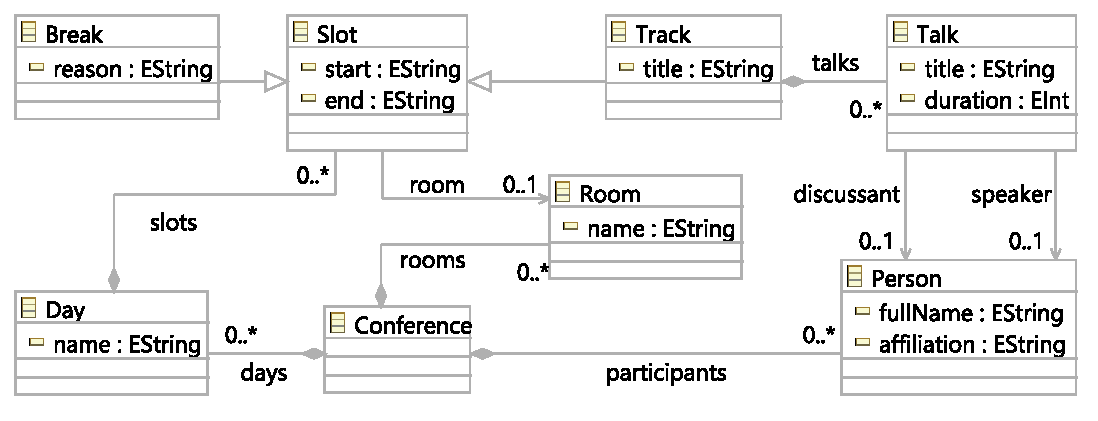
\includegraphics[width=0.9\linewidth]{conference_metamodel}
    \caption{A conference metamodel.}   
    \label{fig:node_metamodel}
\end{figure}

In the evaluation, we introduce a conference metamodel, a more representable metamodel to evaluate the optimised loading. The metamodel has wider EMF feature coverage. It has more than one class (Conference, People, Room, etc. classes) and it applies inheritance. Figure \ref{fig:node_metamodel} shows its metamodel. We need to use contrived example because as a new approach there are no real-world change-based models available. 

\subsection{Saving Time}
\label{subsec:saving_time_test}
We evaluate the performance of our prototype on saving time to gain insight on the efficiency that can be gained from the optimised CBP against the non-optimised CBP and XMI as the comparison baselines. The comparison is depicted in Fig. \ref{fig:append_speed}.

We seek the relationship between number of elements in a model and the time required to persist the model. We create courses of random operations in Epsilon Object Language \cite{kolovos2006epsilon} for each tree and conference domains and executed them to simulate the development of models. In the random operations, we set the probability of different types (create, set, unset, add, move, delete) of operations to occur to 10:1:1:1:1:1 respectively. Such configuration is selected because we want the model to grow faster while other operations are still executed. Since the conference metamodel has several classes (Person, Day, Room, Break, Track, Talk), we set ratio 40:1:3:6:8:24 respectively for them to be created in the \emph{create} operation to ensure that the model is generated proportionally and closer to the the real-world conference models. We start with an empty and execute the random operations to grow the model. Along the growing of the model, we count the number of the elements. Every increase in 100 elements, we measure the time. For  the optimised and non-optimised CBPs, we measure the time consumed to append events generated for each operation, while for XMI, we measure the time used to persist the eventual state of the model after each operation. Also, we check the equivalence of the model loaded from the CBPs against its XMI format to ensure that our approach produces the correct  model.

\begin{figure}[ht]	
    \begin{subfigure}[t]{0.5\linewidth}
		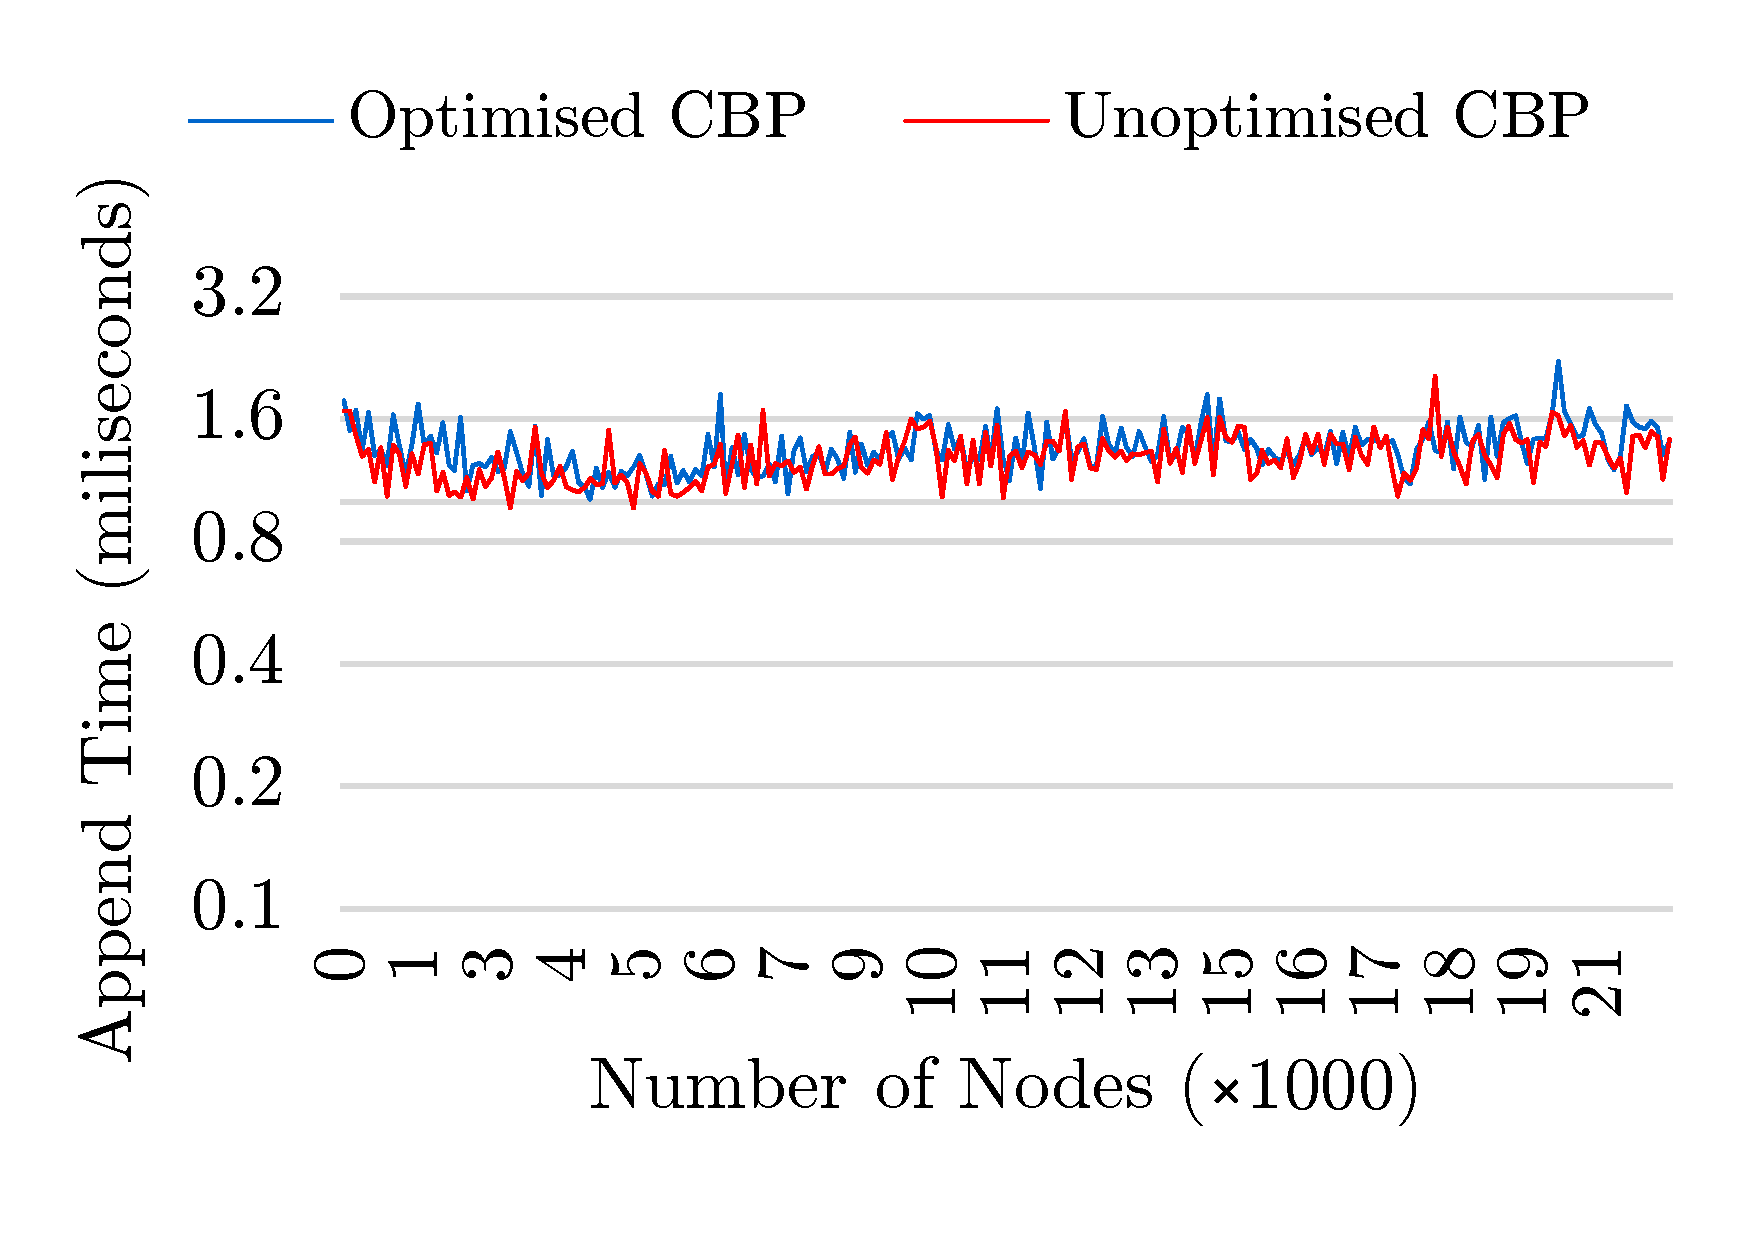
\includegraphics[width=\linewidth]{append_speed_conf}
		\caption{Optimised vs non-optimised CBPs}\label{fig:append_speed_conf}
	\end{subfigure}
	\hfill
	\begin{subfigure}[t]{0.5\linewidth}
		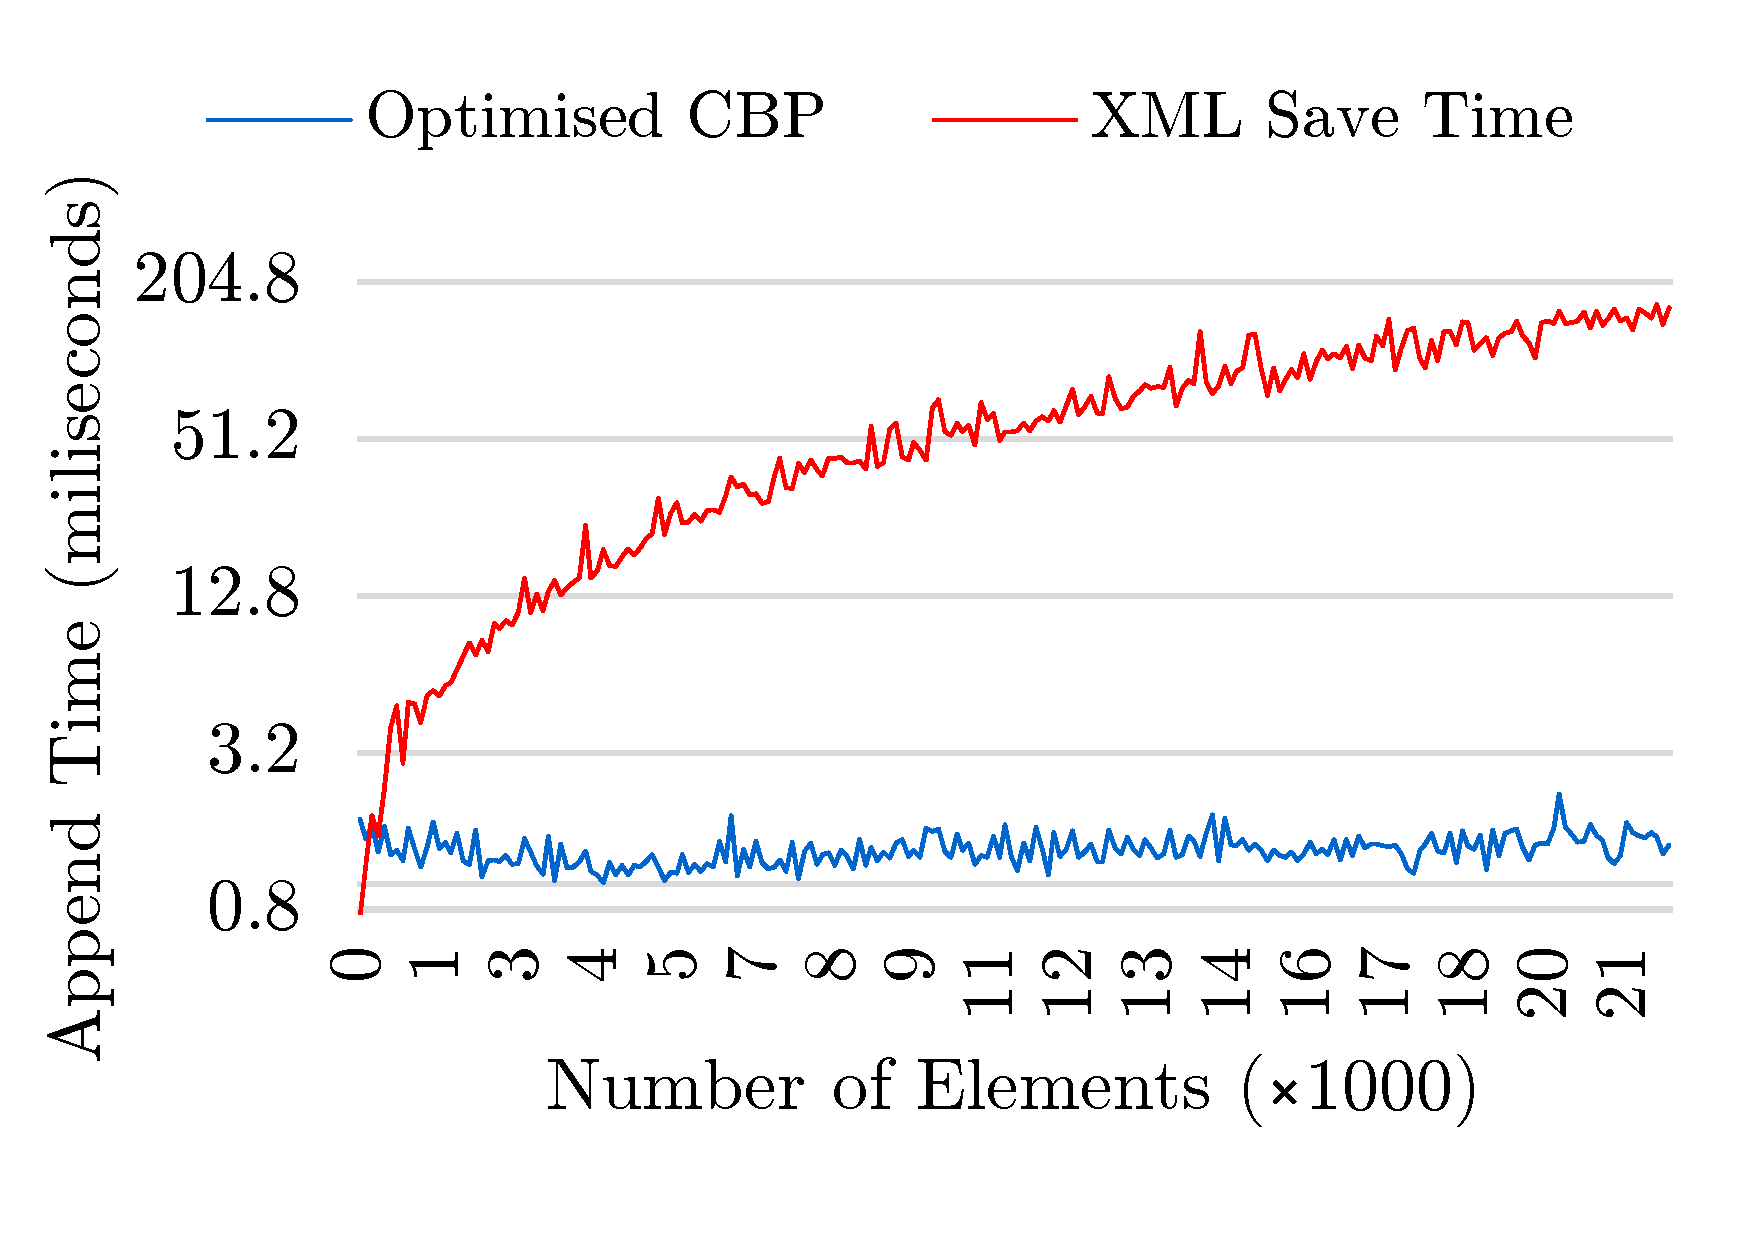
\includegraphics[width=\linewidth]{append_speed_conf_ocbp_xmi}
		\caption{Optimised CBP vs XMI}\label{fig:append_speed_conf_ocbp_xmi}		
	\end{subfigure}	
	\caption{A comparison on time used to persist models between optimised CBP, non-optimised CBP, and XMI. The y-axis is $log_2$ scaled.}
	\label{fig:append_speed}
\end{figure}

In Fig. \ref{fig:append_speed_conf}, the time consumed to persist events in both CBPs is nearly constant, whereas for XMI, the time consumed to persist a model increases linearly along the growth of elements (Fig. \ref{fig:append_speed_conf_ocbp_xmi}). The append time of optimised CBP is slightly higher than the non-optimised CBP's since it has to perform extra computation to populate the \emph{ModelHistory} and \emph{IgnoreList}. Based on our measurement, the average time to append in optimised and non-optimised CBPs is 1.83 and 1.33 miliseconds respectively. The average time required to save model in XMI is increased 6.22 microseconds for every additional element. This finding suggests persisting changes of a model is significantly faster than persisting its complete eventual state after the model is modified.    

\subsection{Loading Time}
\label{subsec:loading_time_test}
We compare optimised CBP, non-optimised CBP, and XMI on their loading time to evaluate the performance of the optimisation algorithm. The  comparison is depicted in Fig. \ref{fig:loading_speed}. We seek the relationship between number of elements of a model and time required to load it. 

In performing the simulation, we create initial elements for the model and generate a number of random operations (create, set, unset, add, move, delete) to manipulate it. The number of the random operations is as many as the number of the initial elements. Also, the probability of the different types of operations to occur is set to 1:1:1:10:5:1 respectively. The probability of \emph{add} and \emph{move} operations are set to 10 and 5 because in a conference typically tracks and talks are of often shifted between days and slots. We start with 7 elements and then increase the number of the initial elements by 500 for each next iteration. For conference model, since it has several classes (Person, Day, Room, Break, Track, Talk), we set ratio 40:1:3:6:8:24 respectively for them to be created in the initial elements and \emph{create} operation to ensure that the model is generated proportionally and closer to real-world conference models. For both CBPs, we measure the time to replay all its events. For XMI, we measure the time consumed to load its model. At the end of each iteration, we check the equivalence of the model loaded from the CBPs against its XMI format to ensure the correctness of the loaded model.

\begin{figure}[ht]	
    \begin{subfigure}[t]{0.5\linewidth}
		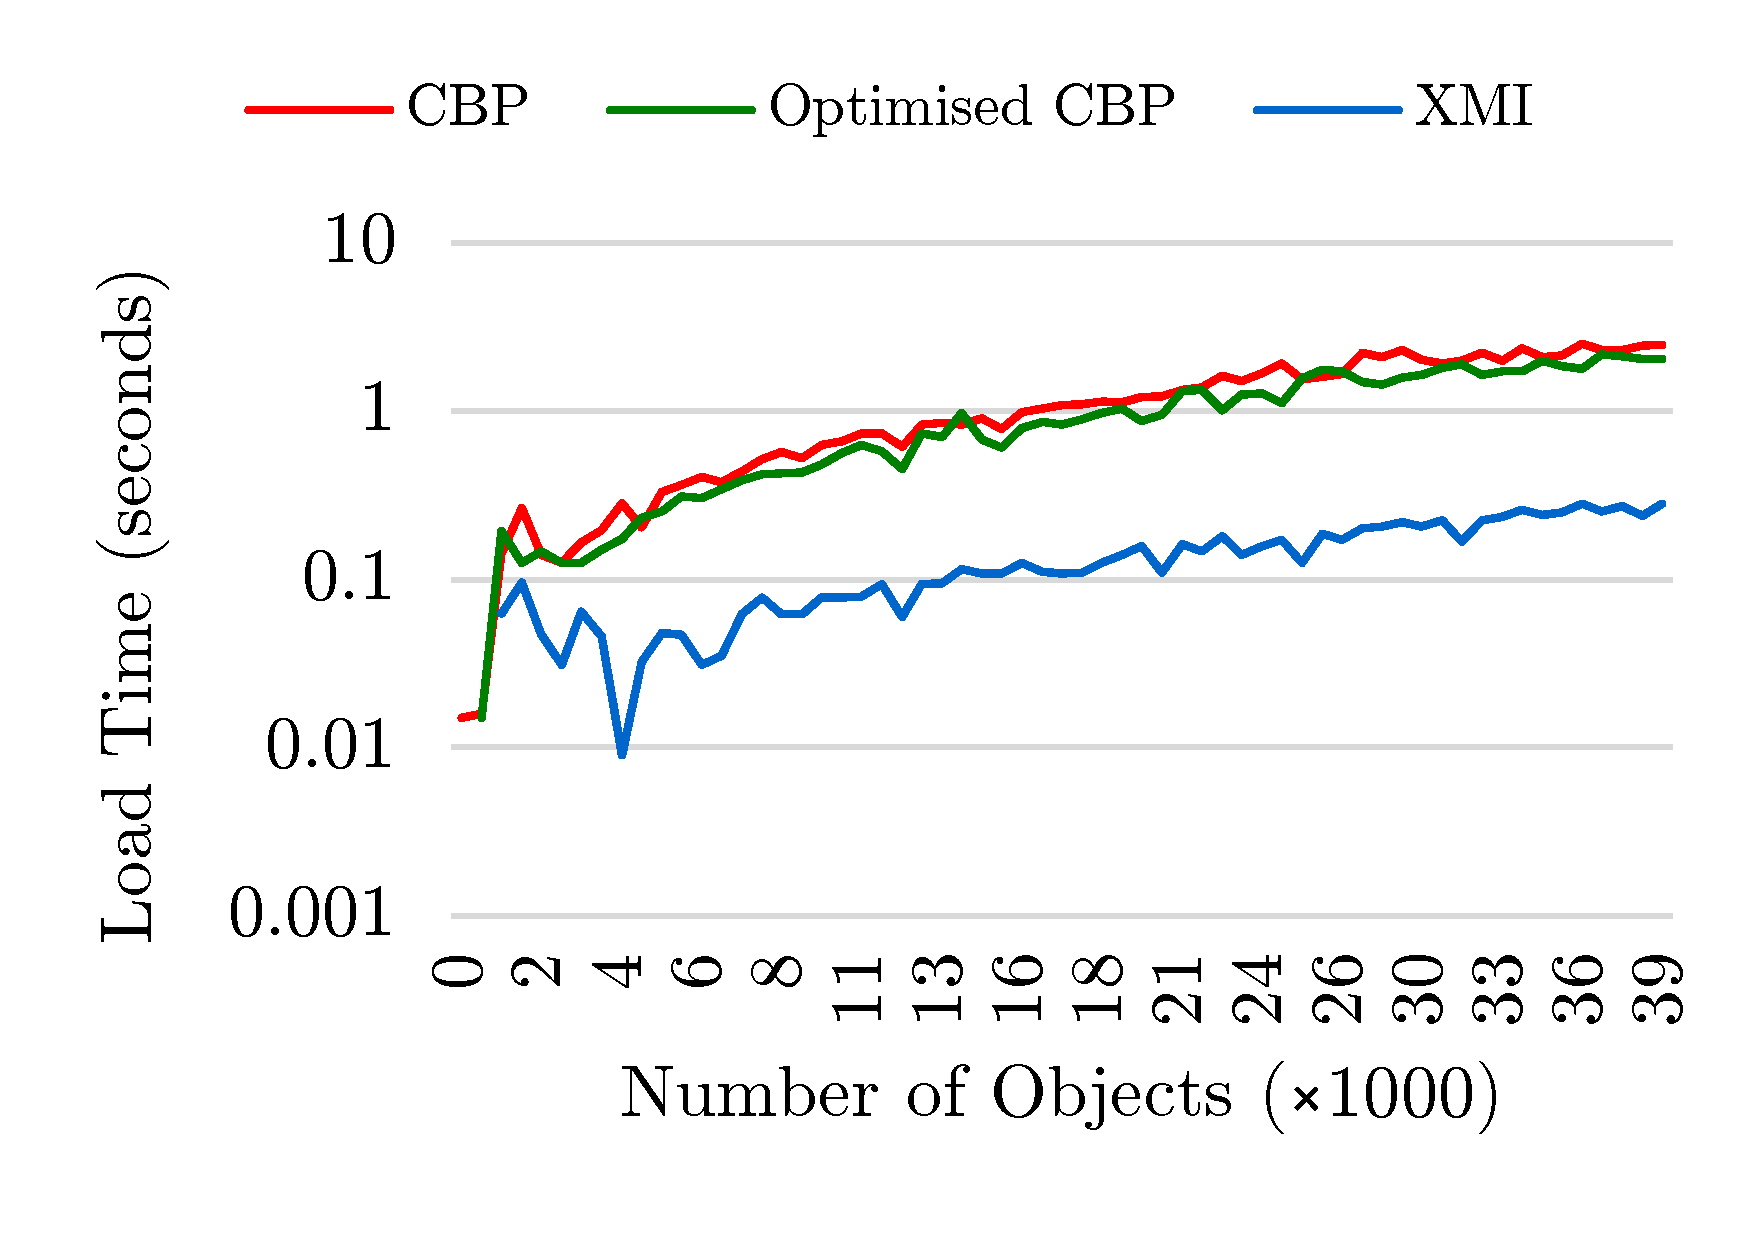
\includegraphics[width=\linewidth]{loading_speed_conf}
		\caption{Optmised CBP vs Non-optimised CBP}\label{fig:loading_speed_conf}
	\end{subfigure}
	\hfill
	\begin{subfigure}[t]{0.5\linewidth}
		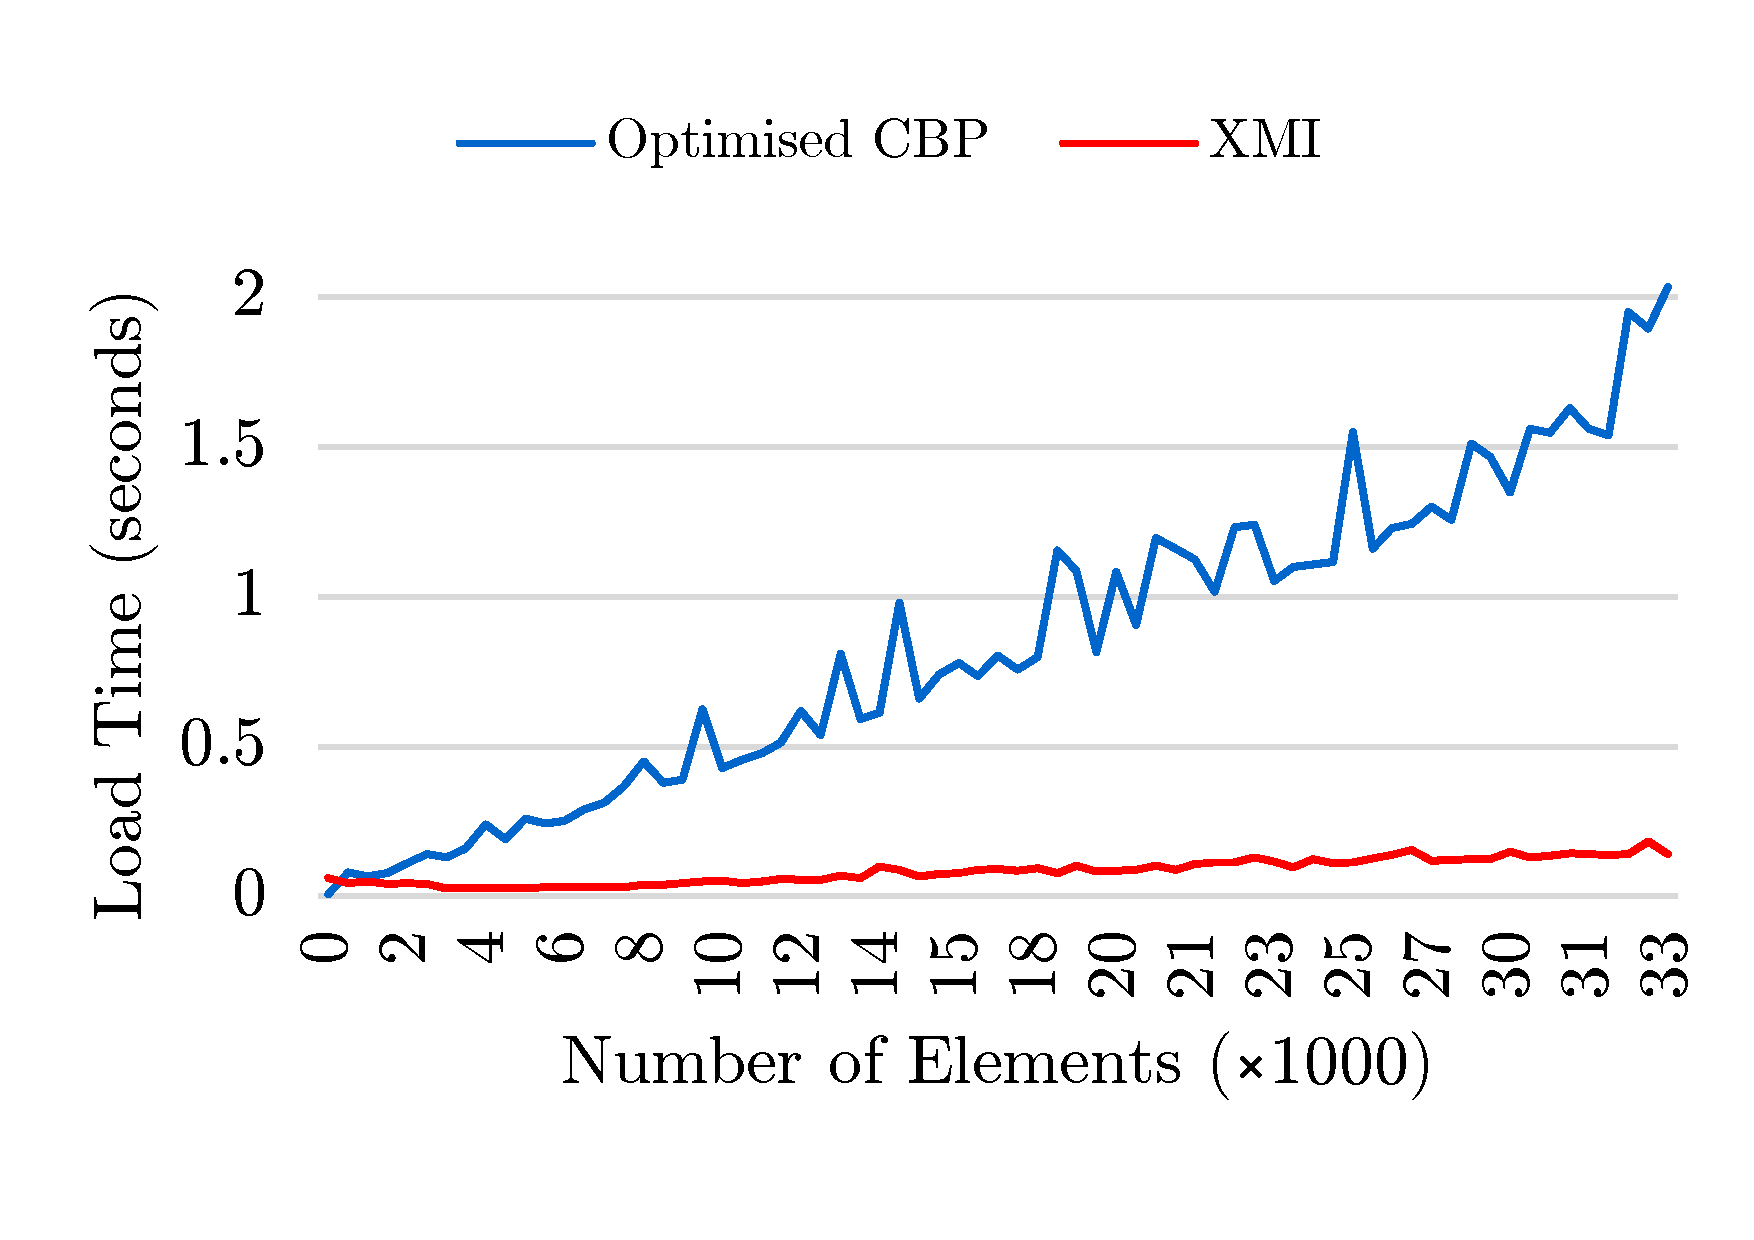
\includegraphics[width=\linewidth]{loading_speed_conf_ocbp_xmi}
		\caption{Optimised CBP vs XMI}\label{fig:loading_speed_conf_ocbp_xmi}		
	\end{subfigure}	
	\caption{A comparison on load time between optimised CBP, non-optimised CBP, and XMI.}
	\label{fig:loading_speed}
\end{figure}

Fig. \ref{fig:loading_speed_conf} shows a pattern that the optimised CBP consumes less time than the non-optimised CBP on loading model. Even though the optimised CBP is faster than the non-optimised CBP on loading models, still it is outperformed by XMI (Fig. \ref{fig:loading_speed_conf_ocbp_xmi}) since it is state-based---no need to replay the construction of its models. For XMI, from our measurement, we obtain that it takes only 5 microseconds in average to load each element in a model. Thus, an XMI with 33,440 elements can be loaded in 0.165 seconds, around 10 times faster than optimised CBP which takes 1.6 seconds for the same number of elements. 

%Based on our investigation, we found out that the time cost of removing an element from a containment reference (delete or move/add it to another reference) of an EMF model grows linearly with the number of elements that it directly contains. So, it is more time consuming to remove an element from a containment reference that has hundreds of members than remove it from a reference that only has ten members. This happens in the three model where a node can contain many other nodes, while in the conference model the proportion of its containment (a day can contain tracks and breaks, a track can contain talks) is kept balanced by the configuration of probability of the instantiation of its classes that is set before. That is why the loading time of the non-optimised CBP in the tree model grows more exponential than the one in the conference model. Thus, the performance of the optimisation on loading time against the non-optimised CBP depends on the structure of models, types of operations that frequently executed, and the amount of operations executed to modify models (more efficiency can be gained if a model is frequently modified).       
         
\subsection{Memory Consumption}
\label{subsec:memory_consumption}

We also compare optimised CBP, non-optimised CBP, and XMI on their memory consumption after loading models. We seek the relationship between number of elements of a model and memory used to after loading the model. The results are shown in Figure \ref{fig:memory_use}. In performing the simulation, we performed the same procedure as in the loading time evaluation (subsection \ref{subsec:loading_time_test}), except for the increment and the dimension that we measure. We set the increment to 100, and instead of measuring the loading time, we measure the memory consumption by subtracting the memory after loading a model with the memory before loading the model.   

Figure \ref{fig:memory_use_conf_ocbp_xmi} shows that optimised CBP consumes more memory than non-optimised CBP, while XMI performs a slightly better than non-optimised CBP in terms of memory saving (Fig. \ref{fig:memory_use_conf_cbp_xmi}). The large memory consumption of optimised CBP is caused by the ignore list which is used for checking events in a CBP if they can be ignored for replay or not. %This condition leads us to another future work that is to identify and remove elements, events, and events numbers from the model history once they are not any longer required. For example, once a element is deleted from a model, all its records in the model history are removed to release space in memory. 

\begin{figure}[ht]	
	\begin{subfigure}[t]{0.5\linewidth}
		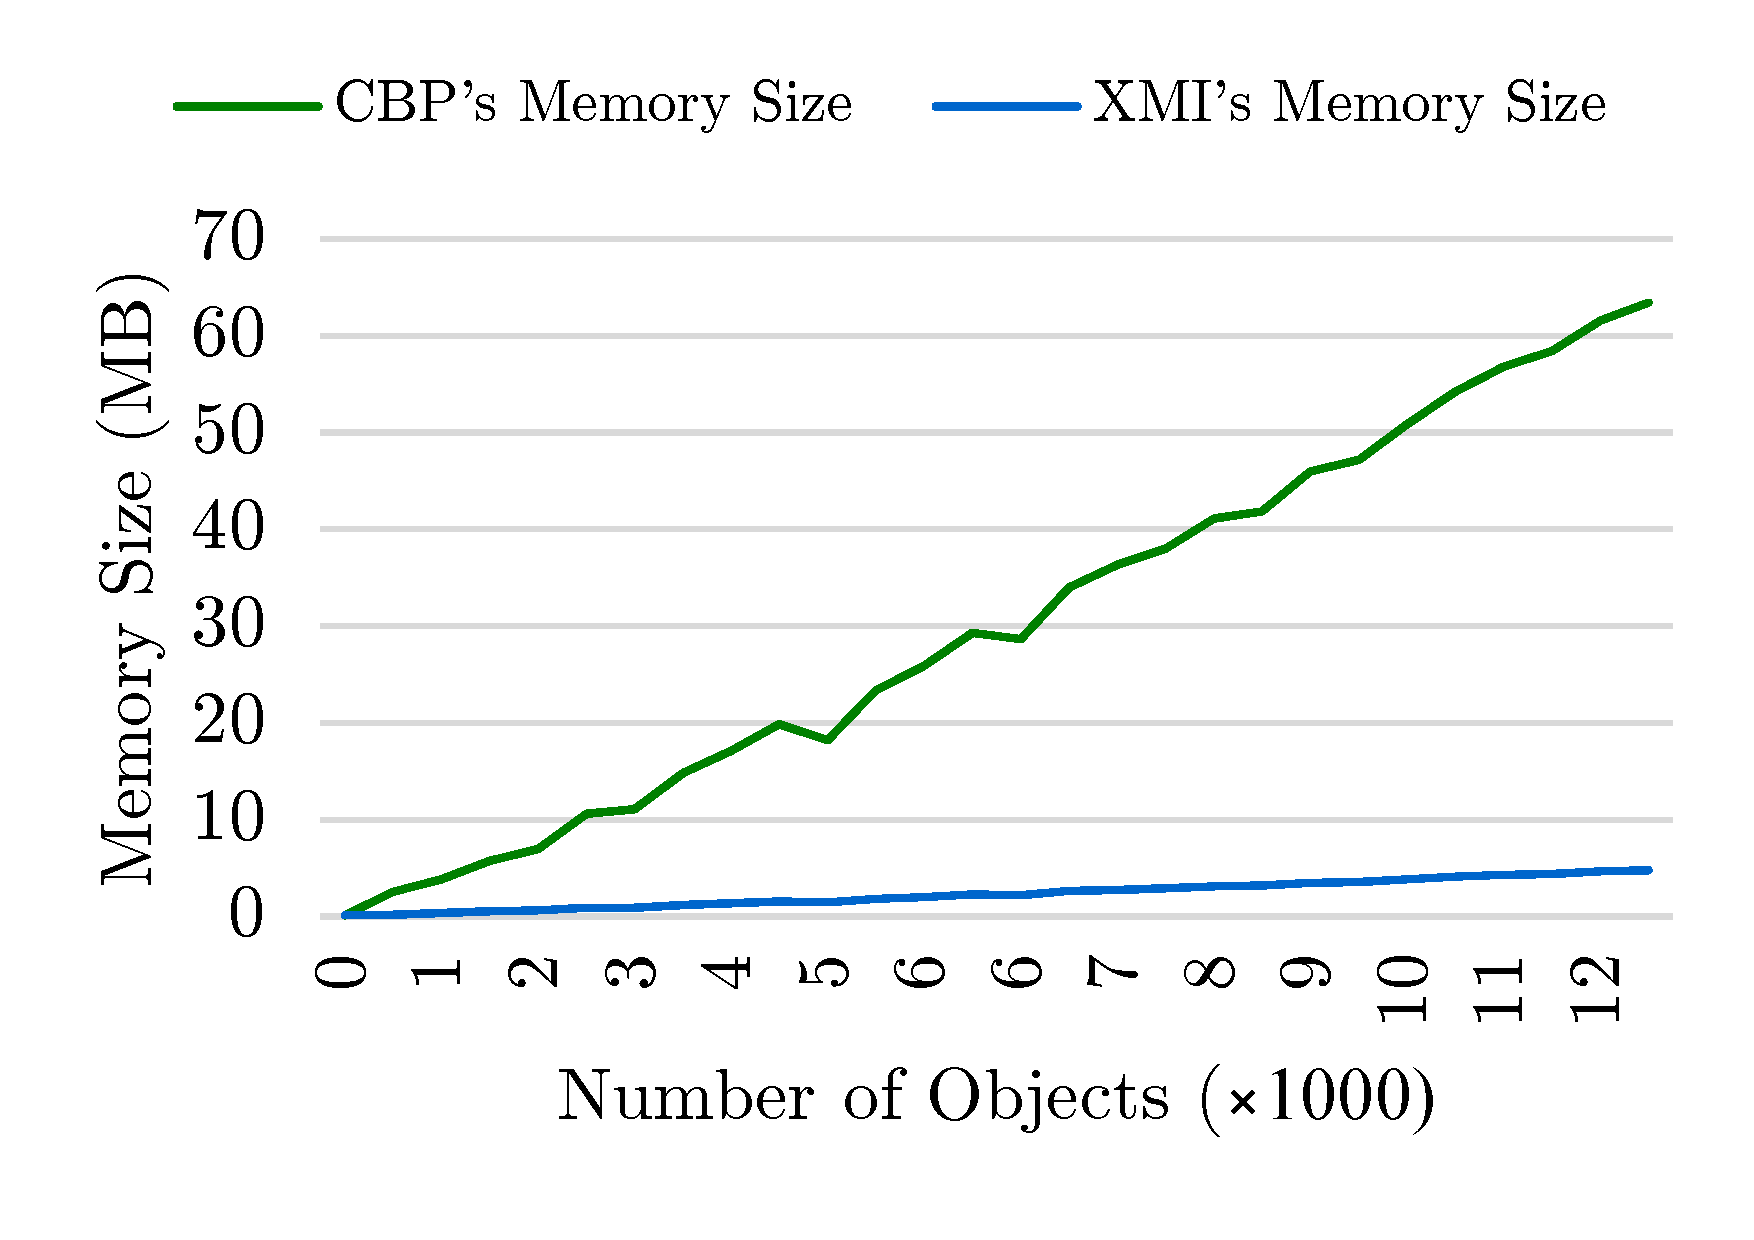
\includegraphics[width=\linewidth]{memory_use_conf}
		\caption{Optimised vs non-optimised CBPs}\label{fig:memory_use_conf_ocbp_xmi}		
	\end{subfigure}
	\hfill
	\begin{subfigure}[t]{0.5\linewidth}
		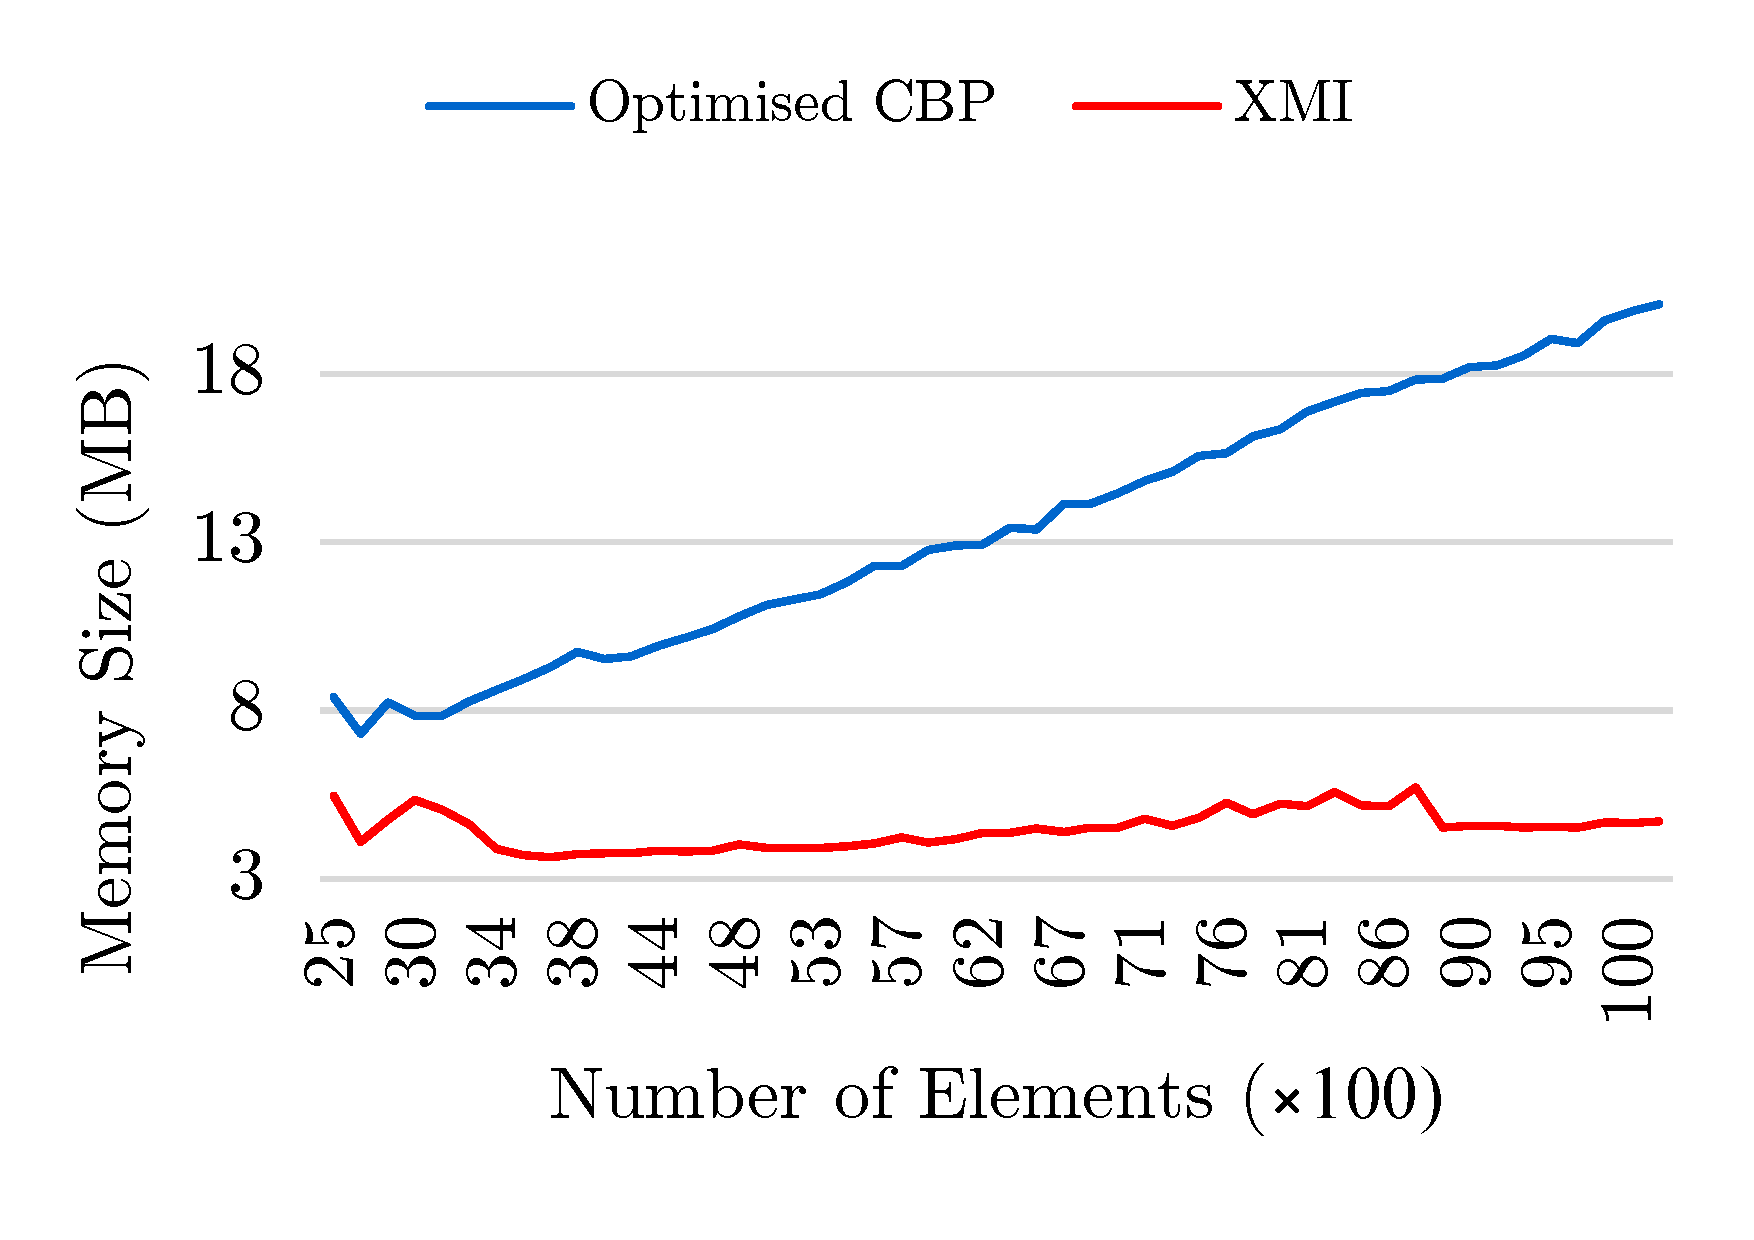
\includegraphics[width=\linewidth]{memory_use_conf_cbp_xmi}
		\caption{Non-optimised CBP vs XMI}\label{fig:memory_use_conf_cbp_xmi}
	\end{subfigure}
	\caption{Memory consumption of optimised CBP, non-optimised CBP, and XMI.}
	\label{fig:memory_use}
\end{figure}

\section{Related Work}
\label{sec:related_work}
Several works have been done in persisting large models , and most of them use databases (e.g. relational, NoSQL). Connected Data Objects (CDO) \cite{eclipse2017cdo} and EMF Teneo \cite{eclipse2017teneo} reduces resources and the time needed to parse XMI documents by persisting models into relational databases. This approach uses metamodels to generate the relational schemas of models and provides  high-level abstraction API for developers to interact with the databases but has drawbacks due to the expensive joins of many tables for highly interrelated models \cite{barmpis2014evaluation}.    
Morsa \cite{pagan2011morsa} uses MongoDB \cite{mongodb2017what}, a NoSQL database, to persist models as a collection of documents by storing every element of a model and its metamodel as entries in an index document that refer to the root elements of their documents. However, due to the nature of the document-based database, storing model's references as serialised documents limits its query and insertion performance as large models have many references which makes them highly interrelated \cite{barmpis2014evaluation}. NeoEMF \cite{daniel2016neoemf} is a prototype that uses several types of NoSQL databases to persist models and lazy-loading mechanism to improve accessing, loading, and removing model elements. Nevertheless, it has not addressed the issues of collaboration, versioning, and fast model differencing. EMFStore \cite{koegel2010emfstore} is a version control system (VCS) that stores changes of models as operations applied to the models, which facilitates collaboration and identify changes of models easier. However, support to use its operation-based approach with more common VCSs (e.g. GitHub, SVN) is not yet available. Several papers mention it does not scale \cite{pagan2011morsa,kolovos2013research} and no optimisation has been proposed to arrive at the eventual versions of models, except replaying all stored operations. 

\section{Limitations and Future Work}
\label{sec:limitations_and_future_work}
So far, we only address feature that can only contain unique members---no duplicate values or elements. Duplicate members means that removal of a value/element does not mean the removal of other same values/elements since values/elements with different positions contained in the feature are perceived different. Therefore, we can update Alg. \ref{alg:add_remove_move_optimisation} to take positions of values/elements as one of its parameters to filter lists of \emph{Line} (Alg. \ref{alg:add_remove_move_optimisation}, lines 6-7). We also have not addressed features that has default values. Default value of a feature might not trigger any event. Failure to address this might produce different eventual models. 

Models in the real world are most likely different from the random models generated in the evaluation. Their optimised CBP's loading can consume more or less time than the ones presented in this paper. There are conditions that the optimised CBP does not always outperform the non-optimised CBP. One condition where optimised CBP is not faster than the non-optimised CBP that is when only \emph{create} operation that is performed, without performing other types of operation, since there is no event that can be ignored. One feasible way to better reflect real-world models is to ask modellers to construct complex models using different modelling languages, persist their histories, scale them up, simulate the loading optimisation, and analyse the results to gain insight whether the optimisation really works for real-world models. 

Since our prototype consumes significant amount of memory in executing the algorithm and still performs more than 10 times slower than XMI in loading models, number of approaches has been identified to reduce memory consumption and loading time. The first approach is optimising the format of CBP so that it consumes less memory and can be parsed faster. The second approach is persisting all events into databases therefore can reduce the use of main memory and NoSQL databases can be considered to improve the loading performance. The third approach is to develop a hybrid persistence representation that is a combination of state-based and change-based persistence. The NeoEMF \cite{daniel2016neoemf} has been successfully implemented NoSQL databases to handle large-scale, state-based model persistence. We plan to extend it to support change-based persistence. Moreover, we also plan to extend the CBP to enable change detection, model merging, conflict resolution of models in the context of collaborative modelling.

\section{Conclusions}
\label{sec:conclusions}
In this paper, we have proposed a change-based, as an alternative to stated-based, persistence as an approach to persist a model. We also have proposed the algorithm to optimise its loading time as well evaluated the change-based persistence on saving time, loading time, and memory consumption against the XMI and non-optimised CBP as the baselines. Our results show considerable savings in terms of persisting and identifying changes made to models at an increased---but linear---model loading cost. 

%\subsubsection*{Acknowledgments.} This work was partly supported through a scholarship managed by \emph{Lembaga Pengelola Dana Pendidikan Indonesia} (Indonesia Endowment Fund for Education).

\bibliography{references} 
\bibliographystyle{splncs}

\end{document}
